\documentclass[a4paper, 12pt]{article}
\usepackage{matnoble-doc-en}


\begin{document}

\title{\bf {CHEM400/740: Quantum Mechanics in Chemistry\\ Chapter\#02}} \author{\bf
  \href{http://scienide2.uwaterloo.ca/~nooijen/website_new_20_10_2011/About.html}{Marcel Nooijen}} \date{}
  
\pagestyle{fancy} \fancyhead[L]{\textcolor{PrimaryColor}{CHEM400/740: Quantum Mechanics in Chemistry}} \fancyhead[R]{\textcolor{PrimaryColor}{2021 Winter}}


\maketitle
\tableofcontents

\clearpage


\section{Review Session}
The full electronic Hamiltonian:
\begin{IEEEeqnarray}{rLl}
\hat{H}&=\hat{h}+\hat{V} 
\end{IEEEeqnarray}

\begin{itemize}
	\item The two-electron operator:
\begin{IEEEeqnarray}{rLl}
\hat{V}&=\frac{1}{2}\sum_{i \neq j} \frac{1}{r_{ij}} 
\end{IEEEeqnarray}

	\item The one-electron operator:
\begin{IEEEeqnarray}{rLl}
\hat{h}&=\sum_i \hat{h}(i) 
\end{IEEEeqnarray}
\tab NOTE: sum over all electrons.

	\item The individual one-electron operator includes kinetic energy and potential energy of nuclei and electrons:
\begin{IEEEeqnarray}{rLl}
\hat{h}(1)&=-\frac{1}{2}\nabla_1^2 + v_{(1)}^{\text{Ne}} 
\end{IEEEeqnarray}

\end{itemize}

 Solve the one-electron Schr\"{o}dinger equation:
\begin{IEEEeqnarray}{rLl}
\hat{h}(1)\psi_a(1)=\varepsilon_a \psi_a(1) 
\end{IEEEeqnarray}
\tab NOTE: \\
\tab \tab $a=1,2,3,\cdots,M$ (finite in `finite basis')\\
\tab \tab Add spin: $\psi_c(r_1)\alpha \rightarrow \psi_c(1)$.\\
\tab \tab \tab \quad \quad $\psi_c(r_1)\beta \rightarrow \bar{\psi}_c(1)$.

Any product function:
\begin{IEEEeqnarray}{rLl}
\psi_{\lambda} =\prod_{k\in \lambda} \psi_{a_i}(r_i)\sigma_k 
\end{IEEEeqnarray}
\tab NOTE: \\
\tab \tab $\lambda$ indicates a configuration of the orbitals that are occupied.\\
\tab \tab $\sigma_k$ includes spin up, $\alpha$, and spin down, $\beta$.\\
\tab \tab Each of the product, $\psi_{\lambda}$, is the eigenfunction of Hamiltonian with eigenvalue, $\sum_{i\in \lambda} \varepsilon a_i$.\\


Antisymmetry requirement:
\begin{IEEEeqnarray}{rLl}
|\phi_{\lambda}\rangle &= \hat{A} \psi_{\lambda}  \\
\hat{A} &= \sum_k^{N!} (-1)^{p_k}\hat{P}_k 
\end{IEEEeqnarray}
\indent NOTE: \\
\tab \tab $\hat{A}$ represents antisymmetrization operator.\\
\tab \tab $p_i$ is called the parity of the permutation (0 or 1).\\
\tab \tab $N!$ is the total number of permutation of N electrons.\\
\tab \tab (+) sign: even number of interchanges\\
\tab \tab ($-$) sign: odd number of interchanges.\\

Or use Slater determinants:
\begin{IEEEeqnarray}{rLl}
|\phi_{\lambda}\rangle =|\psi_a(1)\psi_b(2)\cdots \bar{\psi}_i \cdots \bar{\psi}_Z(N)| 
\end{IEEEeqnarray}
\begin{itemize}
	\item [a)] interchange of electron-label.
	\item [b)] interchange of spin-orbitals.\\
	$\Longrightarrow$ The easiest way to label about spin.
\end{itemize}


These are building blocks of electronic structure theory!


\section{Full Configuration Interaction}
\subsection{Orders of the orbitals}
Rewrite the eigenfunction of Hamiltonian: 
\begin{IEEEeqnarray}{rLl}
\hat{H}\psi &= E \psi  
\end{IEEEeqnarray}

Multiply by the phase factor, a complex number:
\begin{IEEEeqnarray}{rLl}
\hat{H} e^{i\psi} \psi &= E e^{i\psi} \psi 
\end{IEEEeqnarray}

NOTE: \\
\tab \tab $e^{i\psi}\psi$ is also the eigenstate.\\
\tab \tab $e^{i\psi}$: arbitrary phase.\\
\tab \tab  even scaling factor $\Longrightarrow$ change norm of the wavefunction, $\psi$.\\

We can order the orbitals, as changing the order in a determinant introduces a sign at most. Including spin, we might also say:
\begin{IEEEeqnarray}{rLl}
|\phi_{\lambda}\rangle =|\psi_a(1)\psi_b(2)\cdots \psi_Z(N_\alpha) \bar{\psi}_{a'}(1)\bar{\psi}_{b'}(2)\cdots \bar{\psi}_Z(N_\beta)\rangle 
\end{IEEEeqnarray}

NOTE:\\
\tab \tab First includes $N_\alpha$ electrons with $\alpha$ orbitals, then $N_\beta$ electrons with $\beta$ orbitals.\\


\begin{itemize}
	\item If we have M spatial orbitals, the number of distinct determinants with $N_\alpha, N_\beta$ is $\bigl(\begin{smallmatrix} M \\ N_\alpha \end{smallmatrix}\bigr)$, $\bigl(\begin{smallmatrix} M \\ N_\beta \end{smallmatrix}\bigr)$. The number of determinants is gigantic. Each of these determinants is eigenstate of $\hat{h} = \sum_i \hat{h}(i)$ with energy, $\sum_i \varepsilon_i$. Also, eigenstates of $\hat{s}_Z = \frac{1}{2} (N_\alpha - N_\beta)$. One has to use correct orbitals!\\
	
	\item If the orbitals are chosen to be orthonormal, these states are orthogonal. To normalize one has to introduce a factor $\frac{1}{\sqrt{N!}}$. (proof later)
\begin{itemize}
\item[1)] Orthonormality of orbitals:
\begin{IEEEeqnarray}{rLl}
\langle \psi_a| \psi_b \rangle &= \int\psi_a^*(\vec{r})\psi_b(\vec{r})d^3r= \delta_{\alpha\beta} 
\end{IEEEeqnarray} 
NOTE:\\
\tab  $\int\psi_a^*(\vec{r})\psi_b(\vec{r})d^3r$ is called overlap integral.
\item[2)] Non-orthonormality of orbitals: 
\begin{IEEEeqnarray}{rLl}
\langle \psi_a| \bar{\psi}_b \rangle &= \langle \psi_a \alpha| \psi_b \beta\rangle =\langle \psi_a| \psi_b \rangle_{\text{spatial}} \underbrace{ \langle \alpha| \beta \rangle}_{0}=0  
\end{IEEEeqnarray} 
NOTE:\\
\tab  Orbitals with different spin are always orthogonal. $\Longrightarrow \langle \alpha| \beta \rangle =0$.
\item[3)] If orbitals satisfy $\hat{h}(1)\psi_a(1)=\varepsilon_a\psi_a(1)$ and $\varepsilon_a \neq \varepsilon_b$, we can get the overlap of the eigenfunctions, $\langle \psi_a |\psi_b \rangle=0$, where $\hat{h}(1)$ is the Hermitian operator.
\item[4)] If orbitals satisfy $\hat{h}(1)\psi_a(1)=\varepsilon_a\psi_a(1)$ and $\varepsilon_a = \varepsilon_b$, we can always make such orbitals orthogonal/ orthonormal, $\langle \psi_a |\psi_b \rangle= \delta_{ab}$, where $\hat{h}(1)$ is the Hermitian operator.\\
Proof: 
\begin{IEEEeqnarray}{rLl}
&\hat{h}(c_1\psi_a+c_2\psi_b) \notag \\
&= c_1\varepsilon_a\psi_a +c_2\varepsilon_b\psi_b \notag \\
&= \varepsilon_a(c_1\psi_a + c_2\psi_b) 
\end{IEEEeqnarray} 
Any linear combination of degenerate orbitals is also eigenstate.\\
$\Longrightarrow$ Use this to create orthonormal set.\\
\end{itemize}
In general, $\langle \psi_a | \psi_b \rangle = \delta_{ab} = \left\{ \begin{array}{rcl}
        1 & a=b \\
        0 &  \mbox{otherwise} 
           \end{array}\right.$
\item The determinants, $|\phi_\lambda \rangle = \frac{1}{\sqrt{N!}}\hat{A}(\psi_a(1)\cdots \psi_Z(N)) $, use orthonormal basis for Hilbert space. In many-electron system, creating the orthonormal basis is convenient to consider and calculate, hence $\langle\phi_\lambda | \phi_\mu \rangle = \delta_{\lambda\mu}$.
\end{itemize}


\subsection{Two-electron Interaction}
Inclusion of electron repulsion in Hamiltonian:
\begin{IEEEeqnarray}{rLl}
\hat{V}=\frac{1}{2}\sum_{i \neq j} \frac{1}{r_{ij}}
\end{IEEEeqnarray} 
\tab Application of the linear variation principal: the full configuration interaction(CI) model of quantum chemistry.\\
\tab The eigenstates of one-electron Hamiltonian can be used as a basis to set expansion functions for the true many-electron problem. Then, we can make linear combination: 
\begin{IEEEeqnarray}{rLl}
|\psi\rangle=\sum_{\lambda} c_\lambda | \phi_\lambda \rangle
\end{IEEEeqnarray} 
\tab NOTE:\\
\tab \tab The $c_\lambda$ are coefficients to be determined.\\
\tab \tab The $|\phi_\lambda\rangle$ form an in principal complete basis.\\
\tab To obtain the coefficients we can apply variational principal. We need to get the expectation value of the Hamiltonian (energy) and minimize the energy.
\begin{IEEEeqnarray}{rLl}
\frac{\langle \psi |\hat{H}|\psi\rangle}{\langle \psi| \psi\rangle} = \langle H\rangle = E
\end{IEEEeqnarray} 
\tab This leads to a matrix eigenvalue problem. More details see Materials: “Modern Quantum Chemistry” Chapter\#1 (Szabo and Ostlund).
\begin{IEEEeqnarray}{rLl}
\sum_{\mu}\langle \phi_\lambda |\hat{H}|\phi_\mu\rangle c_\mu &=E c_\lambda \\
H C &= C E
\end{IEEEeqnarray} 
\begin{itemize}
\item The orthonormal basis has no overlap matrix.
\item The Equation (20) is the Heisenberg version of Quantum Mechanics. This is also called ``matrix-mechanics".
\item Compared with the Schr\"{o}dinger equation, $\hat{H}\psi = E \psi$, both equations are equivalent and need to solve matrix eigenvalue problem. The Schr\"{o}dinger equation is called ``wave-mechanics".
\item In actual research, we never use Sch\"{o}dinger equation. The research always uses matrix-eigenvalue equations to calculate by computers. This becomes a nice problem in linear algebra.
\end{itemize}

\tab This presents the best solution within the basis set.

\subsection{Excited Determinants and Full Configuration Intereaction}
If we assume we have M orbitals of both $\alpha$ spin and $\beta$ spin. This is determined by basis set used tp expand orbitals.
\begin{IEEEeqnarray}{rLl}
&M \tab \mbox{spatial orbitals} \notag \\
&N_\alpha \tab \alpha \mbox{ electrons} \notag \\
&N_\beta \tab \beta \mbox{ electrons} \notag \\
&(N_\alpha-N_\beta )= 2 \langle S_Z \rangle
\end{IEEEeqnarray} 

The number of determinants / the number of coefficients: 
\begin{IEEEeqnarray}{rLl}
\left( \begin{array}{c} M \\ N_\alpha \end{array} \right)  \cdot \left( \begin{array}{c} M \\ N_\beta \end{array} \right)
\notag
\end{IEEEeqnarray} 
\begin{itemize}
	\item Choose $N_\alpha$ $\alpha$-orbitals out of $M$.
	\item Choose $N_\beta$ $\beta$-orbitals out of $M$.
\end{itemize}
\tab Example for ethylene:\\
\tab\tab\tab	$M \approx$ 100\\
\tab\tab\tab		$N_\alpha \approx$ 10 = $N_\beta$\\
\tab\tab\tab	$ \bigl(\begin{smallmatrix} 100 \\ 10 \end{smallmatrix}\bigr)= \frac{100 \cdot 99 \cdots 91}{10 \cdot 9 \cdots 1} \approx \bigl(\begin{smallmatrix} 100 \\ 10 \end{smallmatrix}\bigr) ^{10} = 10^{10}$\\
\tab	The number of determinants = $10^{10} \times 10^{10} =10^{20} $\\
\tab	The number of matrix-elements = $\langle \phi_\lambda |\hat{H}|\phi_\mu\rangle \approx 10^{20}\cdot 10^{20} = 10^{40}$

Absolutely impossible to store Hamiltonian matrix, let alone diagonalize. Even to store solution, $c_\mu$, is impractical / impossible.\\

This is called full CI solution, such calculations are done for small molecules or small basis sets.
\begin{itemize}
	\item FCI: In principle, the full CI is exact solution in complete one-particle basis
\begin{itemize}
\item [-] Exact solution in finite / small basis set.$\Longrightarrow$ A rigorous benchmark to compare against.
\item [-] Conceptually simple. Insight in solutions to S.E.
\item [-] Only requires $\langle \phi_\lambda |\hat{H}|\phi_\mu\rangle$. Rest in linear algebra can be used in computer science.
\end{itemize}
	\item CAS-CI: Take small set of `active' orbitals and `active' electrons. Next, do Full CI for subproblem. Combine CAS-CI with other methods, like: DFT, perturbation theory, and coupled cluster. These methods can be excellent for very hard problems.
\end{itemize}
It is evident one needs to make approximations. We will see how to do this without loosing accuracy (much).


\section{Hartree-Fock Approximation}
This is a cornerstone of most wave function based on electronic structure approaches. $|\psi_{HF}\rangle$ is approximated by a single determinant, $|\phi\rangle$. Choose the orbitals $\psi_a, \psi_b, \cdots, \psi_Z$.
\begin{IEEEeqnarray}{rLl}
|\phi\rangle = \frac{1}{\sqrt{N!}}|\psi_a(1)\psi_b(2)\cdots \psi_Z(N) |
\end{IEEEeqnarray} 
\tab The orbitals are optimized such that the energy is minimized. Hence, the energy for full Hamiltonian, $\langle \phi |\hat{H}| \phi \rangle $ is minimum. We do not solve for one electron, like $\hat{h}\psi_a = \varepsilon_a \psi_a$, because they do not take into account the repulsion between electrons and electrons, $\hat{V}_{ee}$. Also, orbitals are orthonormal, $\langle \psi_a | \psi_b \rangle =\delta_{ab}$. \\
\tab I will briefly state the equations of Hartree-Fock approximation, we will discuss in more details later.\\
\tab Firstly, expand the molecular orbitals in basis set and introduce a finite atomic basis set, $|\chi_\mu\rangle$. We might choose basis set 6-31g(d,p) or cc-pvtz in Gaussian as an input to do some calculations (fixed by nuclear configurations).
\begin{IEEEeqnarray}{rLl}
\psi_a(1) = \sum_{\mu}\chi_\mu(1)c_{\mu a}
\end{IEEEeqnarray} 
\tab Molecular orbitals are linear combinations of atomic orbitals.\\
\tab Here are some important quantities in AO-basis we can calculate:
\begin{itemize}
	\item Overlap integral:
\begin{IEEEeqnarray}{rLl}
\langle \chi_\mu | \chi_v \rangle = S_{\mu v}
\end{IEEEeqnarray} 
	\item One-electron integrals:
\begin{IEEEeqnarray}{rLl}
\langle \chi_\mu |\hat{h}| \chi_v \rangle = \hat{h}_{\mu v} = \int \chi_\mu^*(1) \hat{h}(1) \chi_v(1) d1
\end{IEEEeqnarray} 
	\item Two-electron integrals:
\begin{IEEEeqnarray}{rLl}
\langle \chi_\mu \chi_v |\frac{1}{r_{12}} | \chi_\lambda \chi_\sigma \rangle \equiv \langle \mu v | \lambda \sigma \rangle = \int \chi_\mu^*(1) \chi_v^*(2)\frac{1}{r_{12}}\chi_\lambda(1) \chi_\sigma(2) d1d2
\end{IEEEeqnarray} 
NOTE: \\
\tab $\chi_\mu$ indicates spin-orbital here.\\
\tab We can also use round brackets to describe two-electron integral, $(\mu\lambda|v \sigma )$. They are same integral. 
\begin{IEEEeqnarray}{rLl}
\underbrace {(\mu\lambda|v \sigma )}_{(11|22)} = \underbrace{ \langle \mu v | \lambda \sigma \rangle }_{\langle 12|21\rangle}
\end{IEEEeqnarray} 
\item Anti-symmetrized two-electron integrals:
\begin{IEEEeqnarray}{rLl}
\langle \mu v || \lambda \sigma \rangle = \langle \mu v | \lambda \sigma \rangle - \langle \mu v |\sigma  \lambda \rangle 
\end{IEEEeqnarray} 
\end{itemize}
\tab These AO-integrals are calculated at the start of a calculation.\\
\tab A Hartree-Fock calculation follows Self-consistent procedure.\\

\subsection{Self-consistent Procedure}
	Assume a guess for molecular orbitals, the molecular coefficient, $C_{\mu i}$ ($i=1, N$ and $\mu = 1, N$).
	\begin{itemize}
		\item [1)] Calculate density matrix for occupied orbitals: 
\begin{IEEEeqnarray}{rLl}
D_{\mu v} =\sum_{i=1,N} C_{\mu i}C_{vi}
\end{IEEEeqnarray} 
		\item [2)] Calculate Fock-matrix: 
\begin{IEEEeqnarray}{rLl}
F_{\mu v}= \hat{h}_{\mu v}+ \sum_{\lambda \sigma}\langle \mu\lambda || v \sigma\rangle D_{\lambda \sigma}
\end{IEEEeqnarray} 
		\item [3)] Solve (generalized) eigenvalue problem: 
\begin{IEEEeqnarray}{rLl}
\sum_v F_{\mu v}C_{vi} = \sum_{\lambda}S_{\mu\lambda}C_{\lambda i}\varepsilon_i
\end{IEEEeqnarray} 
		$\Longrightarrow$ Molecular orbitals $C_{vi}$, Orbital energies $\varepsilon_i $
	\end{itemize}
	\tab If new orbitals ($C_{vi}$) from step 3) agree with input orbitals ($C_{\mu i}$), they are converged. The converged result is the correct HF solution.\\
	\tab Otherwise go back to step 1). Iterate until $F, D, C$ no longer change.\\
	\tab This is called a self-consistent filled procedure.\\
	\tab At self consistency, $D^{(\mbox{in})} \longrightarrow F\longrightarrow \mbox{Diagonalize} \longrightarrow D^{(\mbox{out} )} $. When $D^{(\mbox{in})}= D^{(\mbox{out} )} $, the energy of determinant is optimal (stationary).
	
	In practice one uses smart converge techniques. HF calculations are cumbersome sometimes. \\
\tab NOTE (More discussion later):
\begin{itemize}
	\item [-] The determinant in HF is unique (up to a phase).
	\item [-] The density matrix is unique (given the basis set).
	\item [-] Molecular orbitals are not unique. 
\begin{IEEEeqnarray}{rLl}
\sum_i C_{\mu i}^* C_{vi} =D_{\mu v}
\end{IEEEeqnarray}
One can ritate occupied orbitals.
\begin{IEEEeqnarray}{rLl}
\sum_i C'_{\mu i}=C_{\mu j} u_{ji}
\end{IEEEeqnarray}
Note that the $u_{ji}$ is unitary.
\end{itemize}


Hartree-Fock in practice:
\begin{itemize}
	\item [-] Decent results for geometry optimization (small basis set).
	\item [-] Reasonable harmonic frequencies.
	\item [-] Very poor for thermo chemistry, energy differences.
	\item [-] Not good for potential energy surface.
\end{itemize}


However, total energies in HF are remarkably accurate.
\begin{IEEEeqnarray}{rLl}
E_{\text{HF}} \gtrapprox 99.5\% \text{ of } E_{\text{FCI}} 
\end{IEEEeqnarray}
\tab Total energies are huge. For this reason HF by itself is not good enough. One needs to go beyond: inclusion of electron correlation. Also, HF calculation is often the starting point.



\section{Symmetry in Quantum Mechanics}
This us a vast topic. I wish to discuss have the general principles. I will not go into full detail. In a next section, I will discuss the permutation group, angular momentum and spin.
\subsection{General Principal of Symmetry}
Suppose that we know the solutions to the S.E.
\begin{IEEEeqnarray}{rLl}
\hat{H}|\phi_n\rangle &= E_n|\phi_n\rangle \\
\langle \phi_n|\phi_m \rangle &=\delta_{nm}
\end{IEEEeqnarray}
\tab These solutions form an orthonormal basis for the Hilbert space.\\
\tab Question: \\
\tab Can I find operators $\hat{u}$ such that $\hat{u}|\phi_n\rangle$ also form an orthonormal basis, while having the same energies $E_n$? 
\begin{IEEEeqnarray}{rLl}
(|\phi_m\rangle)^\dagger = \langle \phi_m| &\qquad \hat{u}^\dagger \hat{u}=1 \\
(\hat{u}|\phi_m\rangle )^\dagger \hat{u}|\phi_n\rangle &=\langle\phi_m|\hat{u}^\dagger \hat{u}| \phi_n\rangle =\delta_{mn} \\
\hat{H}\hat{u}|\phi_n\rangle &= E_n\hat{u} |\phi_n
\end{IEEEeqnarray}
\tab NOTE:
\begin{itemize}
	\item [1)] The orthonormal condition implies:
\begin{IEEEeqnarray}{rLl}
\langle\phi_m|\hat{u}^\dagger \hat{u}| \phi_n\rangle = \langle \phi_m | \phi_n \rangle
\end{IEEEeqnarray}
	 $\hat{u}$ is a unitary operator: $\hat{u}^\dagger \hat{u}=1$ and $\hat{u}^\dagger=\hat{u}^{-1}$. Note that the unitary operators preserve orthonormality of a basis, which means $\hat{u}^\dagger \neq \hat{u}$ in general and $\hat{u}^{-1} \neq \hat{u}$ in general. \\
	 \fbox{ Reflection in a plane is its own inverse.} \\
	 Unitary in linear algebra preserves angles and length of a set of vector when general rotation.\\
	 In physics some symmetries are anti-unitary (time-reversal) then $\langle u \phi|u \psi\rangle = \langle \phi|\psi \rangle ^*$ This is not our usual inner product.
	\item [2)]$\hat{u}$ commutes with $\hat{H}$.
\begin{IEEEeqnarray}{rLl}
\hat{H}( \hat{u}|\phi_n\rangle) &= (\hat{u}|\phi_n\rangle )E_n \notag \\
&= \hat{u} \hat{H}|\phi_n\rangle  \qquad \forall \phi_n \\
\hat{H} \hat{u} &= \hat{u} \hat{H}\\
	\left[ \hat{H},\hat{u} 	\right] &=0
\end{IEEEeqnarray}	
This is true for all $|\phi_n\rangle$.
	\item [3)] If $\hat{u}$ commutes with $\hat{H}$, then also $\hat{u}^\dagger = \hat{u}^{-1}$.
\begin{IEEEeqnarray}{rLl}
\hat{H} \hat{u} &= \hat{u} \hat{H} \\
\hat{u}^{-1}\hat{H} \hat{u} &= \hat{u}^{-1} \hat{u} \hat{H} =\hat{H} \\
\notag \\
\hat{u}^{-1}\hat{H} (\hat{u} \hat{u}^{-1}) &= \hat{H} \hat{u}^{-1} \\
\hat{u}^{-1}\hat{H} &= \hat{H} \hat{u}^{-1} \\
\hat{u}^{\dagger}\hat{H} &= \hat{H} \hat{u}^{\dagger} 
\end{IEEEeqnarray}	
	\item [4)] If $\hat{u}_1$ and $\hat{u}_2$ commute, and unitary, then also $\hat{u}_1\hat{u}_2$.
\begin{itemize}
\item [a)]$\hat{H}\hat{u}_1\hat{u}_2 = \hat{u}_1\hat{H}\hat{u}_2 = \hat{u}_1\hat{u}_2 \hat{H}$
\item [b)] $(\hat{u}_1\hat{u}_2)(\hat{u}_1\hat{u}_2)^\dagger = \hat{u}_1\hat{u}_2 \hat{u}_2^\dagger \hat{u}_1^\dagger =\hat{u}_1 \hat{u}_1^\dagger =1 $\\
NOTE:\\
\tab $\hat{u}_1^\dagger\hat{u}_2^\dagger\hat{u}_1\hat{u}_2 \neq 1$
\end{itemize}
	\item [5)] Linear operators are associative.
\begin{IEEEeqnarray}{rLl}
\hat{u}_1(\hat{u}_2 \hat{u}_3) = (\hat{u}_1 \hat{u}_2 )\hat{u}_3 =\hat{u}_1 \hat{u}_2 \hat{u}_3 
\end{IEEEeqnarray}
Always holds for matrix multiplication.\\
It follows that the (full) set of symmetry operations $\hat{u}_i$ form a mathematical group.
\end{itemize}

\subsection{Group}
Definition of a group:\\
\tab Set elements $\{g_i\}$ form a group iff:
\begin{itemize}
	\item [1)] $g_i g_j \in g$ if $g_i$ and $g_j$ is $g$.
	\item [2)] $g_i(g_jg_u)=(g_i g_j)g_u=g_ig_jg_u$   \quad (Associative)
	\item [3)] $hat{I} \in g$, \quad $g_i \cdot \hat{I} = \hat{I}\cdot g_i = g_i$
	\item [4)]$g_i^{-1} \in g$, \quad $g_i^{-1}\cdot g_i =\hat{I}$
\end{itemize}
\tab The theory of groups $\Longleftrightarrow$ The theory of symmetry\\


 More details about Groups (Mathematical):\\
\tab See Link:  \href{https://en.m.wikipedia.org/wiki/Group_(mathematics)}{Wikipedia Website Link on Groups (Mathematical)} \\

Example of a group(1):\\
\tab Elements of $z$ $\{0, \pm 1,\pm 2, \pm 3 \}$.\\
\tab\tab $g_i \otimes g_j$, $\otimes$ means group multiplication.\\
\tab\tab $z_i+z_j$ \\
\tab Whole numbers from a group under addition:\\
\tab\tab $z_1, z_2$ \quad $z_1+z_2 \in Z$\\
\tab\tab $z_1+(z_2+z_3)$ Associative \\
\tab\tab $\hat{I} =0$ \tab \tab $0+z_1=z_1$\\
\tab\tab $z_1+(-z_1)=0 \Longrightarrow \hat{I}$

Example of a group(2):\\
\tab Another group: rational numbers, excluding 0 under multiplication.\\
\tab \tab $x,y \longrightarrow z$ rational \\
\tab \tab $x(x^{-1})=1$, with identity, 1. ($x \cdot 1= 1 \cdot x =1$)\\
\tab \tab  Why is 0 excluded?  $0^{-1} = ?$


\subsection{Example of Groups in Physics}
\begin{tabular}{|c|c|} 
\hline 
Symmetries in physics & Conservation Laws (Noether Theorem) \\
\hline  
Translational & Conservation of Linear Momentum\\
\hline  
Rotations & Angular Momentum is Conserved\\
\hline  
Translation in Time & Conservation of Energy\\
\hline
Rotation of Electron Spin &   Conservation of Spin-angular Momentum\\
\hline
\end{tabular}
\begin{itemize}
	\item Overall translation, $\vec{x} \longrightarrow \hat{T}_a\vec{x}=\vec{x}+\vec{a}$
\begin{IEEEeqnarray}{rLl}
(\hat{T}_a \psi)(\hat{T_a} x)\equiv \psi(x)
\end{IEEEeqnarray}	
NOTE:\\
\tab $\hat{T}_a\psi$: translated function. \\
\tab Translated function in translated point has value of original function in original point.
\begin{IEEEeqnarray}{rLl}
\hat{T}_a ^{-1}\hat{T}_a \psi(\hat{T_a} x) &=\hat{T}_a^{-1}\psi(x) \\
\psi(T_a x)&=\hat{T}_a^{-1} \psi(x)\\
\hat{T}_b &= \hat{T}_a^{-1}\\
\hat{T}_b\psi(x)&= \psi(\hat{T}_b^{-1} x) 
\end{IEEEeqnarray}
This is general definition (Equation 54) of operator on a function, if one knows the operation on coordinates.
\item Overall Rotation (nuclei + electrons)
\begin{IEEEeqnarray}{rLl}
R \psi(x) = \psi(R^{-1}x)
\end{IEEEeqnarray}
Rotations are associated with angular momentum theory, like $\hat{L}_x, \hat{L}_y, \hat{L}_z, \hat{L}^2$. All of angular momentum theory from commutation relations, $[\hat{L}_x, \hat{L}_y] = i \hbar \hat{L}_z$.
\item Multiplication by a phase
\begin{IEEEeqnarray}{rLl}
\psi \rangle = e^{i\phi}|\psi\rangle
\end{IEEEeqnarray}
Same phase for every state.\\
This is origin of gauge theories, electron-magnetism.
\item Permutations of electronic coordinates.
\begin{IEEEeqnarray}{rLl}
\hat{P}_\lambda \psi(x_1,x_2,...,x_N)= \psi(\hat{P}_\lambda^{-1}(x_1,...,x_N))
\end{IEEEeqnarray}
\item Overall rotation of electron spin, for example definition of the z-axis for $s_Z$ operator. \\
This is the conservation of spin-angular momentum. $\hat{s}_z, \hat{s}_x, \hat{s}_y, \hat{s}^2$ commute with the $\hat{H}$. We can use them to build a ``rotation group" in spin space. Analogy to rotation in space, you need to rotate around $4\pi$ to get the identity.

\item Point group symmetry in Chemistry.
If one rotates nuclei and electrons, Hamiltonian is invariant.\\
Now rotate only electronic part of the wave function. Equivalently rotate nuclei in opposite position.
\begin{IEEEeqnarray}{rLl}
\hat{R}\psi(\vec{r}, Q_\alpha ) = \psi(\vec{r},RQ_\alpha )
\end{IEEEeqnarray}
Hamiltonian is invariant under operations. It means nuclei map onto one another.\\
Point group of molecule: 
\begin{figure}[H]
    \begin{subfigure}{.5\textwidth}
        \centering
        % 1
        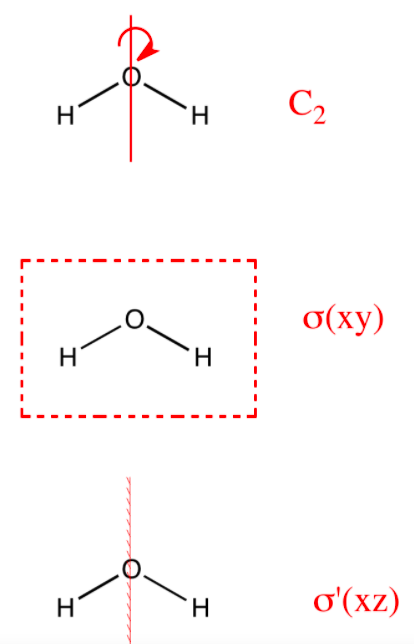
\includegraphics[width=.6\linewidth]{01.png}
        \caption{Water, $C_{2v}$}
        \label{fig:sub-first2}
    \end{subfigure}
    \begin{subfigure}{.5\textwidth}
        \centering
        % 2
        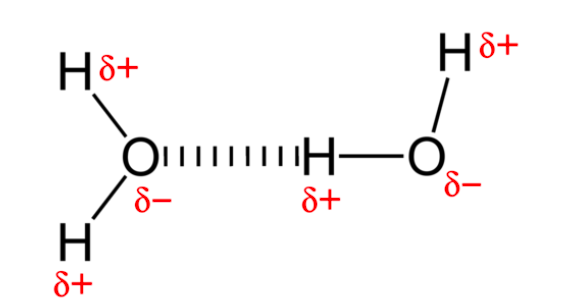
\includegraphics[width=.6\linewidth]{02.png}
        \caption{Benzene, $D_{6h}$}
        \label{fig:sub-second2}
    \end{subfigure}
    \caption{Point Group of Molecules}
    \label{fig:fig2}
\end{figure}
\end{itemize}

 More details about Groups in Physics:\\
\tab See Link:  \href{https://en.m.wikipedia.org/wiki/Group_(mathematics)}{Wikipedia Website Link on Groups in Physics} \\


\subsection{Consequences of Symmetry}

\begin{summary}{}{}
Summary of Symmetry Considerations (Abstract Discussion) 
\begin{itemize}
	\item [1)] Unitary operators preserve orthonormality of a basis.
$$ \hat{u}^\dagger\hat{u}= I ; \hat{u}^\dagger= \hat{u}^{-1}$$
$$\langle \phi_k|\hat{u}^\dagger\hat{u} |\phi_l \rangle = \langle \phi_k|\phi_l \rangle  =\delta_{kl}$$
if original basis is orthonormal. 
	\item [2)] If $\left[ \hat{H}, \hat{u} \right] =0$, then if $\hat{H}|\psi\rangle = E| \psi\rangle$.
$$\hat{H}(\hat{u}|\psi\rangle )= E(\hat{u}|\psi\rangle)$$
$\hat{u}|\psi\rangle$ is eigenstate of $\hat{H}$ with the same energy $E$.
	\item [3)] If unitary $\hat{u}_1, \hat{u}_2$ and $\left[ \hat{H}, \hat{u}_i \right] =0, i=1,2$. Then,
$$\hat{u}_3=\hat{u}_1\hat{u}_2$$
\begin{itemize}
\item [a)] $\hat{u}_3$ is a unitary.
\item [b)] $\hat{u}_3$ commutes with $\hat{H}$.
\end{itemize}
	\item [4)] $\hat{u}^\dagger =\hat{u}^{-1}$ is unitary and commutes with $\hat{H}$.
	\item [5)] $I$ is unitary and commutes with $\hat{H}$.\\
\end{itemize} 
	$\Rightarrow$ The set of symmetry operators $\hat{u}_i$ form a mathematical group.(Statement 2-5: postulates that define a mathematical group.)\\
	$\Rightarrow$ All aspects of group theory (a part of algebra) apply to symmetry in Quantum Mechanics.  
\end{summary}

\tab What if $E_n$ is non-degenerate?

\subsubsection{Example: Particle on a Ring}
The Schr\"{o}dinger equation of a particle on a ring: 
\begin{IEEEeqnarray}{rLl}
-\frac{\hbar^2}{2mR^2}\frac{d^2\psi(\phi)}{d (\phi)^2} &= E \psi(\phi) \\
\hat{H} = -\frac{\hbar^2}{2mR^2}\frac{d^2}{d \psi^2} &= \frac{\hat{L}_z}{2mR^2} \\
\hat{L}_z &=- i\hbar \frac{\partial}{\partial \psi}  \\
I &= mR^2
\end{IEEEeqnarray}


\begin{figure}[H]
        \centering
        % 1
        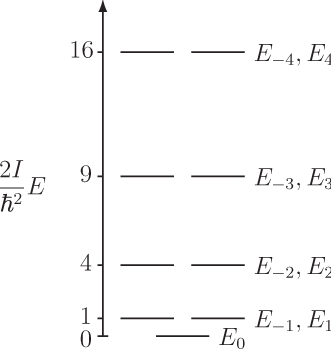
\includegraphics[width=.3\linewidth]{03.png}
        \caption{The energy level of a particle on a ring. }
        \label{fig:sub-first2}
\end{figure}

 The eigenfunctions corresponding to $+m$ and $−m$ are linearly independent, so both must be accepted. Therefore all eigenvalues, except  $E_0$ , are two-fold (or doubly) degenerate. The eigenfunctions can all be written in the form const ​ $e^{ik\phi}$ , with $m$ allowed to take either positive and negative values (or 0).\\
 \tab NOTE: \\
\tab \tab The degeneracy of 2 means that two different wave functions with same eigenvalues. \\
\tab\tab Different wave functions mean more different than overall phase.\\
\tab\tab NOT different: $|\phi_n\rangle \longrightarrow (e^{ik\phi})|\phi_n \rangle$ is also eigenstate.\\
\tab\tab Degenerate states: choose the orthonormal.

General solution: 
\begin{IEEEeqnarray}{rLl}
f(\phi) = c_1 e^{ik\phi}+c_2 e^{-ik\phi}
\end{IEEEeqnarray}

Solutions are not unique. Consider:
 $$  \left\{ \begin{aligned}
         sin (k\phi)\\ cos (k\phi)
            \end{aligned}\right. \qquad \text{or} \qquad  \left\{ \begin{aligned} e^{ik \phi}\\ e^{-ik\phi}
            \end{aligned}\right.$$
\begin{IEEEeqnarray}{rLl}
cos(k\phi) &= \frac{1}{2}(e^{ik\phi}+e^{-ik\phi})\\
sin(k\phi) &= \frac{1}{2}(e^{ik\phi}-e^{-ik\phi})
\end{IEEEeqnarray}

The set of solutions / the subspace of solutions that we choose is unique. 
\begin{summary}{}{}
The solution of a particle on a ring: \\
\indent $\frac{1}{\sqrt{2\pi}}e^{ik\phi}$ and $\frac{1}{\sqrt{2\pi}}e^{-ik\phi}$ are eigenstates of $\hat{H}$ with the same eigenvalue (energy), $\frac{k^2 \hbar^2}{2mR^2} (\frac{k^2 \hbar^2}{2I})$.
Freedom in choice according to different basis sets or different subspaces: 
\begin{itemize}
	\item [a)] Real eigenfunctions:
 $$  \left\{ \begin{aligned}
        \frac{1}{\sqrt{\pi}} sin (k\phi)\\ \frac{1}{\sqrt{\pi}}  cos (k\phi) 
            \end{aligned}\right. \qquad k=0: \frac{1}{\sqrt{2\pi}} $$
	\item [b)] Eigenstates of $\hat{L}_z$:
$$  \left\{ \begin{aligned}
        \frac{1}{\sqrt{2\pi}}e^{ik\phi}\\ \frac{1}{\sqrt{2\pi}}e^{-ik\phi}
            \end{aligned}\right.  $$
	\item [c)] Other choice, for example	:
 $$  \left\{ \begin{aligned}
        \frac{1}{\sqrt{\pi}} sin (k\phi + \alpha )\\ \frac{1}{\sqrt{\pi}}  cos (k\phi+ \alpha) 
            \end{aligned}\right. $$
            $\alpha$ for arbitrary.
\end{itemize}   
\end{summary}



More details about Particle on a Ring, see Link:  \href{http://scienide2.uwaterloo.ca/~nooijen/Chem356/particle_on_the_ring.pdf}{Particle on a Ring}. 



\subsubsection{Consequences of Symmetry: Multiplet}
Consider a multiplet of eigenstates of Hamiltonian, $|\phi_k\rangle$, all with same energy, $E$. The number of orthonormal states is well defined as degeneracy. States themselves are called freedom. The space it spans is always the same. 
\begin{IEEEeqnarray}{rLl}
\sum_{k \in E} |\phi_k \rangle \langle\phi_k =\hat{P}_E
\end{IEEEeqnarray}
\tab NOTE: \\
\tab \tab $\hat{P}_E$ is a projector on this space.\\
\tab Then for any symmetry operator $\hat{u}^a$:
\begin{IEEEeqnarray}{rLl}
\hat{H}(\hat{u}^a|\phi_n \rangle ) &= E_n |(\hat{u}^a| \phi_n \rangle)
\end{IEEEeqnarray}
\tab Hence, $\hat{u}^a$ is a linear combination of states in the multiplet.
\begin{IEEEeqnarray}{rLl}
\hat{u}^a|\phi_l \rangle  &=\sum_{l \in P_E}|\phi_l \rangle \langle\phi_l |\hat{u}^a|\phi_k \rangle \notag \\
&= \sum_{l \in P_E}|\phi_l \rangle\hat{u}^a_{lm}
\end{IEEEeqnarray}
\tab Likewise:
\begin{IEEEeqnarray}{rLl}
\hat{u}^b|\phi_l \rangle &=\sum_{l \in P_E}|\phi_m \rangle\hat{u}^b_{ml}
\end{IEEEeqnarray}
\tab The important point is that $\hat{u}|\phi_k \rangle $ cab always be expressed in terms of the states in the multiplet.\\
\tab $\longrightarrow$ Stay in the subspace.
\begin{IEEEeqnarray}{rLl}
\hat{u}^b\hat{u}^a|\phi_l\rangle &= \sum_{m,l \in P_E} |\phi_m \rangle \langle\phi_m | \hat{u}^b |\phi_l \rangle \langle\phi_l | \hat{u}^a | \phi_k \rangle \\ 
&= \sum_{m,l \in P_E} |\phi_m \rangle \hat{u}^b _{ml}\hat{u}^a _{lk} \\
&\equiv |\phi_m \rangle \hat{u}^{ba} _{mk}
\end{IEEEeqnarray}
\tab It follows that the matrix-elements of the symmetry operator, follow the same multiplication law as the group. 
\begin{IEEEeqnarray}{rLl}
\hat{u}^{ba} &= \hat{u}^b\hat{u}^a \qquad \forall a,b
\end{IEEEeqnarray}
\tab $\Rightarrow$ Group multiplication $\Longleftrightarrow$ Matrix multiplication\\
\tab The dimension of the matrices is the same as degeneracy of Hamiltonian.



\subsubsection{Consequences of Symmetry: Irreducible Representations}
Group theory: The matrices $\hat{u}^a$ form a representation of a group. 

 $\blacksquare$ Example: \\
\tab \tab H-atom : 1s (non-degenerate)\\
\tab \tab Rotations: 1-dimensional matrices (just numbers)\\
\tab  p-orbitals ($p_x, p_y, p_z$) : 3-dimensional matrices (3-dimensional representation).\\
\tab  d-orbitals ($d_{xy}, d_{yz}, d_{xz}, d_{x^2-y^2},d_{z^2}$) : 5-dimensional matrices (5-dimensional representation).\\
\tab  $\Rightarrow$ We get the representations of groups.\\
\tab  $\Rightarrow$ Heart of group theory.

If one cannot reduce the set of functions further, i.e one cannot find a new basis in which all matrices $\hat{u}^a$ have a block form. Then the representation is called irreducible. \\
\tab Functions $|\phi_l\rangle$: transform according to irreducible representations.\\
\tab The eigenstates of the Hamiltonian can always be chosen to transform as irreducible representations of the symmetry group of $\hat{H}$.
\begin{IEEEeqnarray}{rLl}
\phi_n| n, \Gamma, i \rangle
\end{IEEEeqnarray}
\tab NOTE:\\
\tab \tab $\Gamma$: irreducible representation.\\
\tab \tab $i$: column of irrep.\\
\tab \tab $n$: labels different multiplets, different energy $E_n$.
\begin{IEEEeqnarray}{rLl}
y_l^m(\theta, \psi ) \qquad \text{Spherical Harmonics}
\end{IEEEeqnarray}
\tab NOTE:\\
\tab \tab $l$: label of irrep.\\
\tab \tab $m$: different columns of irrep.\\
\tab For many electron atoms, we use the same angular momentum label $S, P, D, F$ and can label functions as $(L,M)$.\\
\tab $\Rightarrow$ irreducible representations (same as orbitals)\\
\tab For molecules: Orbitals and many-electron wave functions transform as irreducible representations: $A_1, B_1, B_2, A_2$ for water, $C_{2v}$ etc.\\
\tab The irreducible representations are determined by the symmetry group. Independent of Hamiltonian. One can show: 
\begin{IEEEeqnarray}{rLl}
\langle \phi_k, \Gamma_1, i_1|\hat{H}|\phi_l, \Gamma_2,i_2\rangle=0
\end{IEEEeqnarray}
\tab NOTE:\\
\tab \tab unless $\Gamma_1=\Gamma_2$ same irrep.\\
\tab \tab unless $\Gamma_1=\Gamma_2$ same column.\\
\tab \tab $k$ labels different functions all transforming as $\Gamma_1, i$\\
\tab Only functions that `interact' have the same symmetry. Interaction means make matrix-elements of Hamiltonian.\\
\tab $\Rightarrow$ The Hamiltonian is block diagonal in a symmetry-adapted basis.

Example (water, $C_{2v}$):
\begin{figure}[H]
        \centering
        % 1
        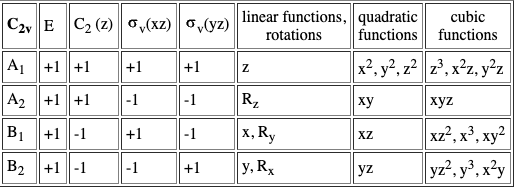
\includegraphics[width=.8\linewidth]{04.png}
        \caption{Character table for point group C2v. }
        \label{fig:sub-first2}
\end{figure}
Only need to diagonalize blocks: cost of diagonalizations  $\thicksim n^3$\\
\tab $h$ blocks: h diagonalizations of $\thicksim n/h$ blocks.
cost, $h(n/h)^3 =\frac{1}{h^2}n^3$.


\fbox{ Symmetry:} 
\begin{itemize}
	\item [a)] Symmetry can be very important to use to make calculation more efficient.
	\item [b)] States can be labelled according to symmetry $\Rightarrow$ qualitative understanding, degeneracy pattern.
\end{itemize} 
\tab The use of irreducible representations is the most elaborate use of symmetry in Quantum chemistry.\\
\tab $\Rightarrow$ It is all `just' group theory (math). Any correct results in math will never change.


More details about Irreducible Representations:\\
\tab See Link:  \href{https://en.m.wikipedia.org/wiki/Irreducible_representation}{Wikipedia Website Link on Irreducible Representations} 





\subsection{Complete Set of Commuting Operators}

Alternate way to think of symmetry: complete set of commuting operators.\\
\tab Let $\hat{A}, \hat{B}$ be Hermitian operators that commute with $\hat{H}$, and also with each other. (unitary operators are usually not Hermitian)
\begin{IEEEeqnarray}{rLl}
[\hat{H}, \hat{A}]=[\hat{H},\hat{B}]=[\hat{A},\hat{B}]=0
\end{IEEEeqnarray}
\tab Example: $\hat{H},\hat{L}^2, \hat{L}_z$

Hermitian operator: $\hat{O}| O_i\rangle =O_i|O_i\rangle$
\tab Get eigenvalues and eigenvectors.\\
\tab Then, we can define a complete set of common eigenstates $|E_n, a_i, b_j \rangle$.
\begin{IEEEeqnarray}{rLl}
\hat{H}|E_n, a_i, b_j \rangle &= E_n|E_n, a_i, b_j \rangle \\
\hat{A}|E_n, a_i, b_j \rangle &= a_i|E_n, a_i, b_j \rangle \\
\hat{B}|E_n, a_i, b_j \rangle &= b_j|E_n, a_i, b_j \rangle
\end{IEEEeqnarray}
\tab Simultaneous, eigenstates of $\hat{H}, \hat{A}, \hat{B}$.\\
\tab If $\hat{A}, \hat{B}$ have complete set of common eigenstates then $\left[ \hat{A},\hat{B}\right]=0$\\
\tab\tab\tab\tab$\left[ \hat{A},\hat{B}\right]=0  \xLeftrightarrow[\text{(2)}]{\text{(1)}}$ complete set of common eigenstates\\
\tab Proof (1):\\
\tab \tab Complete basis: $|\psi=\sum_{i,j}|a_i,b_j \rangle c_{ij}$\\
\tab \tab Any $\psi$ can be expanded in $|a_i,b_j\rangle$
\begin{IEEEeqnarray}{rLl}
\hat{A}\hat{B}|a_i,b_j \rangle &= \hat{A}( b_j|a_i,b_j \rangle) \notag \\
&=  a_ib_j|a_i,b_j \rangle \\
\hat{B}\hat{A}|a_i,b_j \rangle &= \hat{B}( a_i|a_i,b_j \rangle) \notag \\
&= b_j a_i|a_i,b_j \rangle \\
(\hat{A}\hat{B}-\hat{B}\hat{A})|\psi\rangle &=(\hat{A}\hat{B}-\hat{B}\hat{A})\sum_{i,j}|a_i,b_j \rangle c_{ij} \notag \\
&= \sum_{i,j}(a_ib_j-b_ja_i\rangle )c_{ij} =0 \qquad \forall \psi
\end{IEEEeqnarray}
\tab \tab Reverse the order of the eigenvalues, and eigenvalues are numbers.\\
\tab Proof (2):\\
\tab \tab The converse part: if $\left[ \hat{A},\hat{B} \right] =0$, they have a complete set of common eigenstates is most \tab \tab involved, but instructive:\\
\tab \tab First, diagonalize the operator $\hat{B}$:\qquad  $\hat{B}|b_j\rangle = b_j|b_j\rangle $.\\
\tab \tab Reverse order: \qquad $(\hat{B}^\dagger|b_i\rangle )^\dagger = \langle b_i|\hat{B}$. \\
\tab \tab Hermitian operator:\qquad \quad  $\hat{B}^\dagger = \hat{B}$.\\
\tab \tab Eigenvalues of Hermitian operator are real: \qquad $\hat{B}^\dagger =\langle b_i|b_i \rangle)^\dagger =\langle b_i|b_i^* =\langle b_i|b_i $\\
\tab \tab Acting with $\hat{B}$ on bra directly.\\
\tab \tab Analogue: right and left eigenvectors for matrices. \\
\tab \tab For Hermitian/Symmetric matrices  eigenvectors are same (or hermitian conjugate).\\
\tab \tab Eigenvalues are the same.
\begin{IEEEeqnarray}{rLl}
\langle b_i|[\hat{A},\hat{B}]|b_j\rangle &=0 \\
\langle b_i|\hat{A}\hat{B}-\hat{B}\hat{A}|b_j\rangle &=0 \\
(b_i-b_j)\langle b_i|\hat{A}|b_j\rangle &=0 
\end{IEEEeqnarray}
\tab\tab $\Longrightarrow$ If $b_i \neq b_j$, then:
\begin{IEEEeqnarray}{rLl}
\langle b_i|\hat{A}|b_j\rangle &=0
\end{IEEEeqnarray}
\tab\tab $\Longrightarrow \hat{A}$ is block diagonal in $\hat{B}$ basis.\\
\tab\tab Second, diagonalize the $\hat{A}$:
\begin{table}[!htbp]
\centering
\begin{tabular}{|c|c|c|c|}
\hline 
$\hat{A}$ & $b_1$ & $b_2$ & $b_3$\\
\hline  
$b_1$ & x & 0 & 0 \\
\hline 
$b_2$ & 0 & x & 0 \\
\hline 
$b_3$ & 0 & 0 & x \\
\hline 
\end{tabular}
\end{table}\\
\tab\tab $\hat{A}$ is block-diagonal.\\
\tab\tab I can diagonalize each block by itself. This does not change eigenvalue of $\hat{B}$.\\
\tab\tab All states in a $b_i$ block have same eigenvalues.
\begin{IEEEeqnarray}{rLl}
\hat{A}| a_i, b_j \rangle &= a_i| a_i, b_j \rangle \\
\hat{B}| a_i, b_j \rangle &= b_j| a_i, b_j \rangle
\end{IEEEeqnarray}
\tab\tab This procedure can be repeated including additional commuting operators.
\begin{IEEEeqnarray}{rLl}
\hat{B}\sum_k| b_j, k\rangle c_k &= \sum_k b_j| b_j, k\rangle c_k \rangle \notag \\
&= b_j(\sum_k| b_j, k\rangle c_k)
\end{IEEEeqnarray}
\tab Linear combination of states with same eigenvalue $b_j$ is eigenstate of $\hat{B}$ with eigenvalue $b_j$.
\tab If three operators are commuting $\left[ \hat{A},\hat{B} \right]=\left[ \hat{A},\hat{C} \right]=\left[ \hat{B},\hat{C} \right]=0 $, the complete set of eigenstates is $|a_i, b_j, c_k \rangle$.\\
\tab $\Longrightarrow$ These all present good quantum numbers.\\
\tab $\Longrightarrow$ Labels for the states.\\
\tab e.g.  $ \hat{H}, \hat{L}^2, \hat{L}_z \longrightarrow | E_n, l, m \rangle$\\
\tab e.g.  $ \hat{S}_1^2, \hat{S}_z \longrightarrow | E_n, L, M, S, M_s \rangle$\\

In a time-dependent formulation $\langle \hat{A} \rangle$ and $\langle \hat{B} \rangle$ would not depend on time.
\begin{IEEEeqnarray}{rLl}
\langle \psi(t) |\hat{A}|\psi(t) \rangle &= \langle \psi(t=0) |e^{i\hat{H}t}\hat{A}e^{-i\hat{H}t}|\psi(t=0) \rangle \notag \\
&= \langle \psi(t=0) |\hat{A}|\psi(t=0) \rangle
\end{IEEEeqnarray}
\tab $\hat{H}$ is independent of time.
\begin{IEEEeqnarray}{rLl}
[\hat{H},\hat{A}]&=0\\
\frac{d\langle \hat{A} \rangle}{dt}&=0\\
\left[\hat{H} ,f( \hat{A}) \right]&=0 \qquad f(\hat{A})\text{: Taylor series expansion} \\
\left[\hat{H}^n,\hat{A}\right]&=0
\end{IEEEeqnarray}
\tab Such operators represent conserved quantities.\\
\tab Any Hermitian operator that has $\left[ \hat{H},\hat{A} \right]=0$ is a conserved quantity.
\begin{IEEEeqnarray}{rLl}
\hat{A}^\dagger &=\hat{A}\\
(e^{i\hat{A}})^{\dagger} = e^{(i\hat{A})^{\dagger}} &=e^{-i\hat{A}^\dagger}=e^{-i\hat{A}}\\
e^{i\hat{A}}(e^{i\hat{A}})^\dagger &=e^{i\hat{A}}e^{-i\hat{A}} =1
\end{IEEEeqnarray}
\tab NOTE:\\
\tab \tab $\hat{A}$: hermitian operator.\\
\tab \tab $e^{i\hat{A}}$ is a symmetry operator, or even $e^{i\hat{A}\alpha}$ is symmetry operator with real parameter $\alpha$.\\
\tab This is a way to make the connection between symmetries and conserved quantities.\\

Example(1):\\
\tab \tab  $\hat{L}_x, \hat{L}_y, \hat{L}_z$ are hermitian, commute with $\hat{H}$.
\begin{IEEEeqnarray}{rLl}
\hat{L}_{\pm} &=\hat{L}_x+i\hat{L}_y \\
\hat{L}_+|l,m\rangle \longrightarrow c_+|l,m+1\rangle \qquad &\hat{L}_-|l,m\rangle \longrightarrow c_-|l,m-1\rangle \notag \\
\left[\hat{H},\hat{L}_+ \right]&= 0 \\
\left[\hat{H},\hat{L}_- \right]&= 0 
\end{IEEEeqnarray}
\tab \tab $\hat{L}_+,\hat{L}_-$ create new eigenstates with same eigenvalue.\\
\tab \tab $e^{\alpha\hat{L}_x+\beta\hat{L}_y+\gamma\hat{L}_z } $ is an operator that defines wave functions in a rotated frame.\\
\tab \tab These symmetries are continuous symmetries group described by linear algebras.\\

Example(2):\\
\tab \tab  $\hat{p}_x$ commutes with free-particle motion $\hat{h}=-\frac{1}{2}\frac{d^2}{dx^2}$, which means $\left[ \hat{p}_x,\hat{h}\right]=0$.\\
\tab \tab $e^{iahat{p}_x}|\psi(x)\rangle$ creates translated function.
\begin{IEEEeqnarray}{rLl}
e^{ia\hat{p}_x}&=e^{ia\langle-i\hbar\frac{\partial}{\partial x} |}=e^{a\hbar\frac{\partial}{\partial x}} \longrightarrow e^{b\frac{\partial}{\partial x}} \qquad \text{with} \quad b=a\hbar \\
\notag \\
e^{b\frac{\partial}{\partial x}}f(x)&=f(x)+b\frac{\partial f}{\partial x} + \frac{1}{2}b^2\frac{\partial^2 f}{\partial x^2}+\cdots+\frac{1}{n!}b^n\frac{\partial^n f}{\partial x^n} \notag \\
&=f(x+b) 
\end{IEEEeqnarray}
\tab \tab NOTE: Taylor series expansion.


There are many aspects to symmetry. We often perceive symmetry as beautiful. The theory of symmetries is also very beautiful (group theory). For we personally, the study of group theory (independent reading class) was the first made me want to be a `theoretical chemist'.




















\end{document}